\chapter{Introduction}
Consider a robot that navigates the world by the use of its camera sensors.
By tracking how the environment appears to move through a sequence of images (Figure~\ref{fig:keypoint-matches}), it is possible to reconstruct both the motion of the robot relative the world, and a 3D map of the environment (Figure~\ref{fig:sfm}).
\begin{figure}[htb]
    \centering
    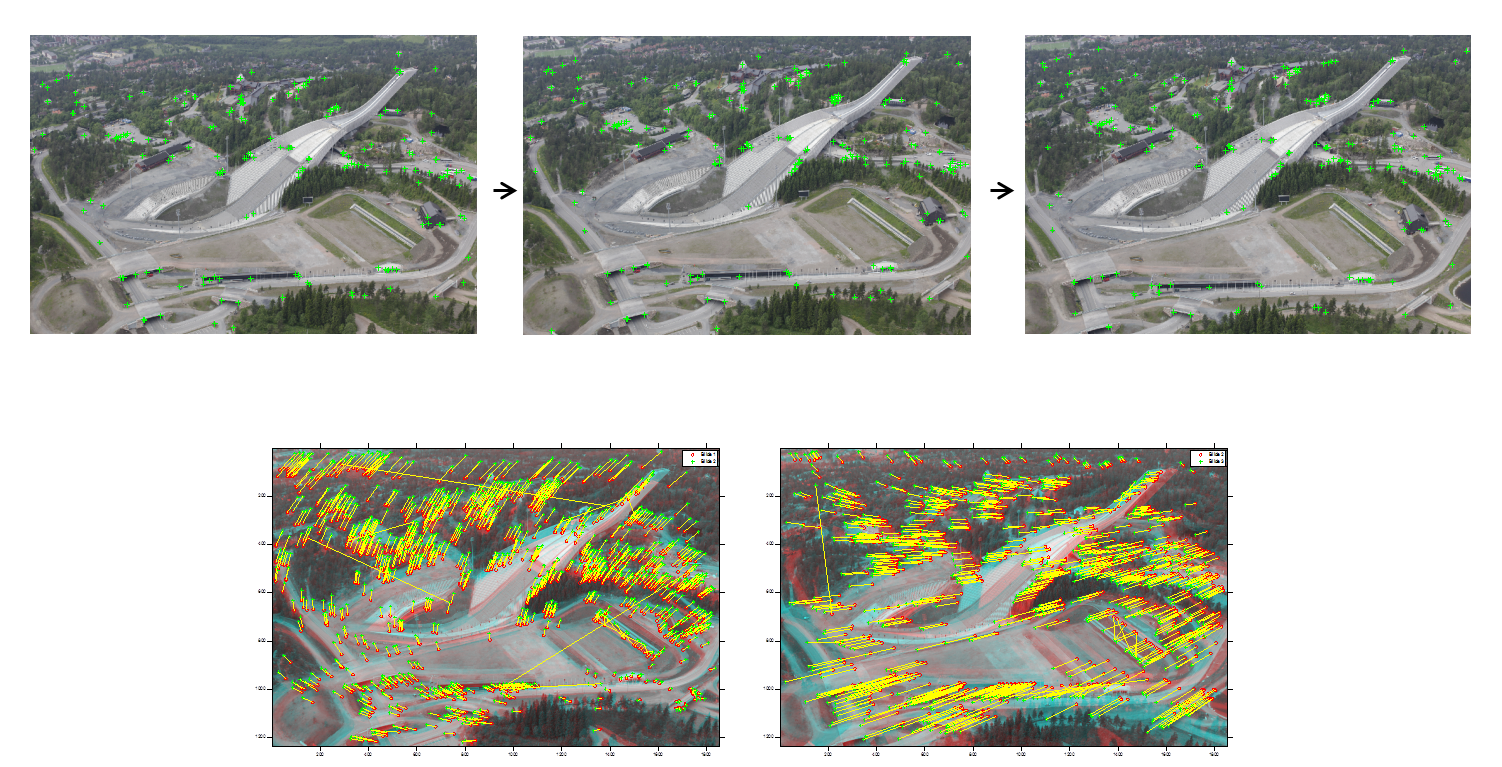
\includegraphics[width=\columnwidth]{figures/keypoint_matches.png}
    \caption{
    Tracking the scene in a sequence of images.
    In the top row, we see an example of how we can repeatedly detect corresponding points in the scene by extracting keypoint features. 
    By computing local descriptors around these points, we can search for putative point matches between the images, such as shown in the bottom row. 
    Outliers can be removed by only keeping matches that fit with the same type of motion hypothesis.
    }
    \label{fig:keypoint-matches}
\end{figure}
\begin{figure}[htb]
    \centering
    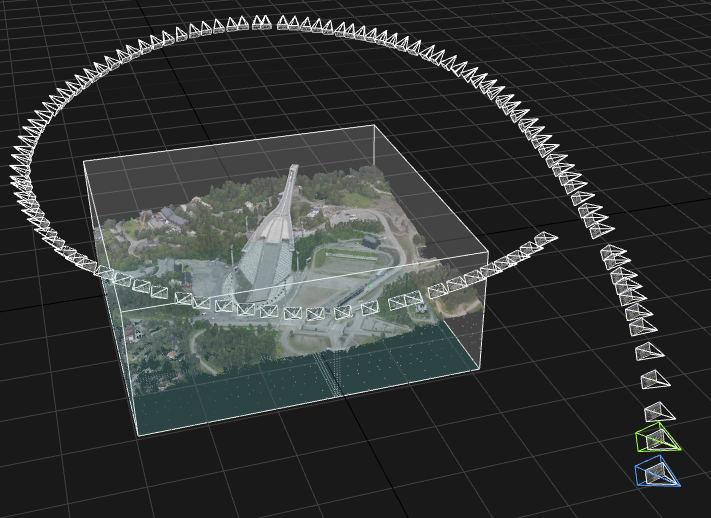
\includegraphics[width=0.75\columnwidth]{figures/holmenkollen-3d.png}
    \caption{An example of estimating motion and a 3D map from a sequence of images.}
    \label{fig:sfm}
\end{figure}

The map can be used to support tasks such as planning robot motion through rough terrain or avoiding obstacles.
It also allows us to limit the error in the motion estimation by serving as a reference for navigation.
By recognising revisited areas and correcting for drift through \emph{loop-closure} constraints, the robot can ``reset'' its localisation error and recover the true topology of the environment, as illustrated in Figure~\ref{fig:topology}.
This approach to navigation is often called \emph{Visual Simultaneous Localisation and Mapping (VSLAM)}.
Approaches that reduce computations and complexity by estimating maps locally without loop-closures are often called \emph{Visual Odometry (VO)} systems, and can be considered as reduced VSLAM systems, with the place recognition module disabled.
Such approaches reduce drift locally, but are unable to correct for drift in the long-term, and will not recover the global topology of the scene.
\begin{figure}[htb]
    \centering
    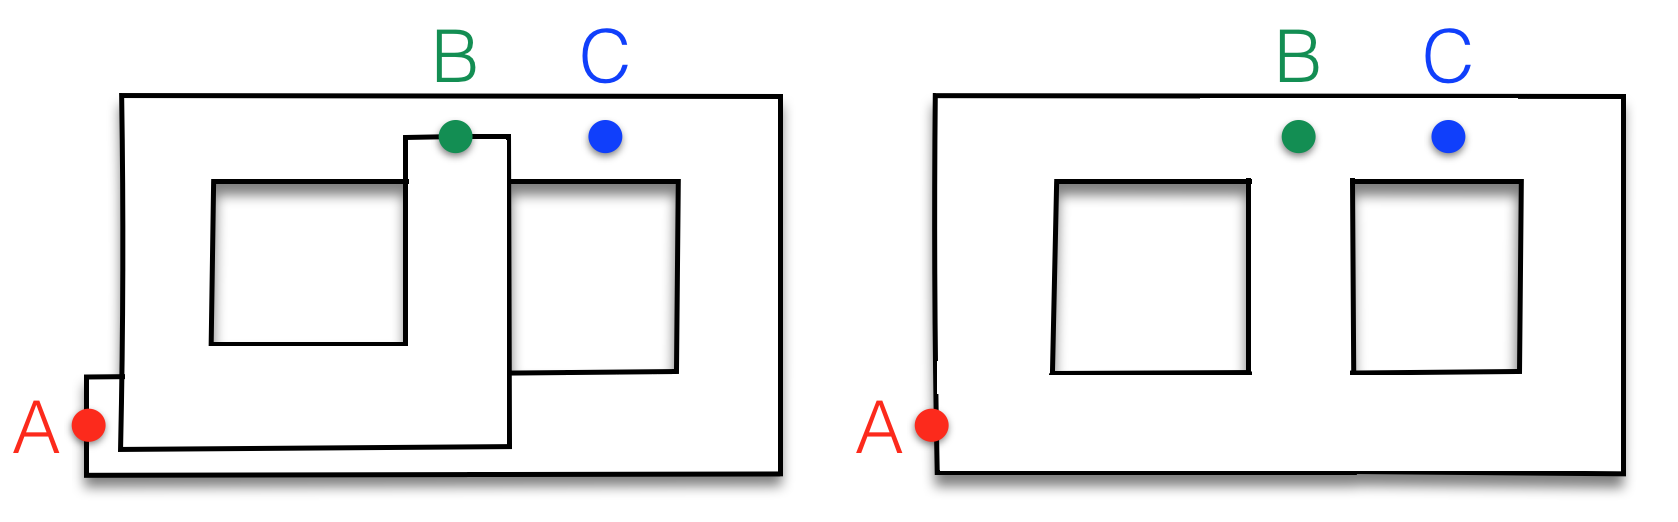
\includegraphics[width=0.75\columnwidth]{figures/topology.png}
    \caption{
    Left: Map built from odometry.
    Points that are close in reality (e.g. B and C) may be arbitrarily far away in the local map.
    Right: By leveraging loop-closures, VSLAM can recover the true topology of the environment, and discover ``shortcuts'' in the map.
    (Image source: \cite{Cadena2016})
    }
    \label{fig:topology}
\end{figure}

\begin{figure}[htb]
    \centering
    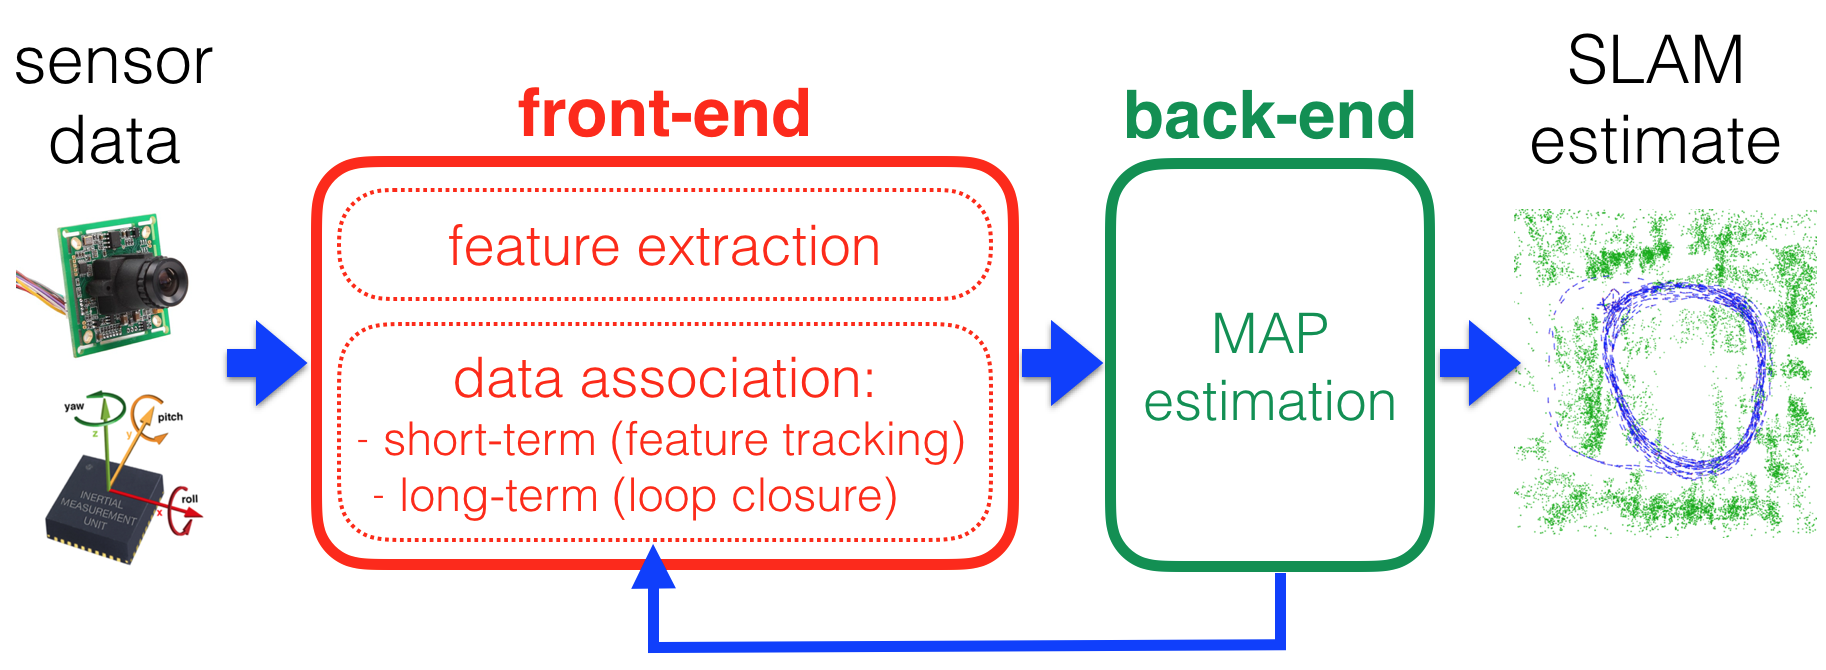
\includegraphics[width=0.75\columnwidth]{figures/frontBack.png}
    \caption{
    Front end and back end in a typical VSLAM system.
    (Image source: \cite{Cadena2016})
    }
    \label{fig:front-and-backend}
\end{figure}
It is customary to separate a SLAM system into two main components: the \emph{front end} and the \emph{back end} \cite{Cadena2016} (Figure~\ref{fig:front-and-backend}).
The front end extracts relevant data from raw sensor measurements, and performs data associations between the measurements and the map.
The back end performs estimation and inference on data from the front end.
Notice that the back end may also incorporate measurements from other types of sensors, such as \emph{inertial measurements units (IMUs)}.
We will here focus on the back end in VSLAM systems.

We may formulate the problem of estimating both motion and structure from noisy sensor measurements by using a Bayesian probabilistic model.
Assume that we want to estimate the unknown set of state variables $X$ that includes both the motion of the camera and the structure of the scene.
Also assume that we are given a set of sensor measurements $Z$ that depend upon the true state of $X$.
The most often used estimator for $X$ is the \emph{maximum a posteriori} (MAP) estimate, which maximises the posterior density $p(X | Z)$ of the states $X$ given the measurements $Z$.
By applying Bayes' law, we get
\begin{align*}
    X^\text{MAP} &= \argmax_X p(X | Z)\\[1em]
    &= \argmax_X \frac{p(Z | X) p(X)}{p(Z)}\\[1em]
    &= \argmax_X l(X;Z) p(X),
\end{align*}
where $l(X;Z) \propto p(Z | X)$ is the likelihood of the states $X$ given the measurements $Z$, defined as any function proportional to $p(Z | X)$.
This can be seen as a form of sensor model, that allows us to evaluate how well the measurements fit with our current hypothesis for the states $X$.
The density $p(X)$ is the prior density over the states, which allows us to evaluate how well our current hypothesis fits with any prior knowledge about $X$.

This handbook is meant to provide a terse, but thorough, introduction to the fundamentals behind how such problems may be expressed and solved.
We will start by covering how we can describe states and sensor models using 3D geometry and Lie theory.
This includes a framework for expressing derivatives of vectors, orientations and poses, and representing uncertainty in such variables.
We will then see how nonlinear least squares can be applied to find the MAP estimate for states, given noisy measurements and corresponding measurement prediction models.
Finally we will cover how this can be applied in estimating pose and structure from images.

Hopefully, this handbook will be useful background when studying Visual odometry and Visual SLAM systems.
